%%%%%%%%%%%%%%%%%%%%%%%%%%%%%%%%%%%%%%%%%%%%%%%%%%
%% Bachelor's & Master's Thesis Template        %%
%% Copyleft by Dawid Weiss & Marta Szachniuk    %%
%% Faculty of Computing and Telecommunication   %%
%% Poznan University of Technology, 2020        %%
%%%%%%%%%%%%%%%%%%%%%%%%%%%%%%%%%%%%%%%%%%%%%%%%%%


% Szkielet dla pracy licencjackiej pisanej w języku polskim.

\documentclass[polish,a4paper,oneside]{ppfcmthesis}


\usepackage[utf8]{inputenc}
\usepackage[OT4]{fontenc}

%--------------------------------------
% Strona tytułowa
%--------------------------------------

% Autorzy pracy, jeśli jest ich więcej niż jeden
% wstaw między nimi separator \and
\author{%
   inż. Jakub Zdanowski \album{127239}
}
\authortitle{}                                % Do not change.

\title{Rozpoznawanie emocji w mediach społecznościowych z wykorzystaniem głębokich sieci neuronowych}

% Your supervisor comes here.
\ppsupervisor{~dr hab.~inż.~Agnieszka Ławrynowicz} 

% Year of final submission (not graduation!)
\ppyear{2020}                                 


\begin{document}

% Front matter starts here
\frontmatter\pagestyle{empty}%
\maketitle\cleardoublepage%

%--------------------------------------
% Miejsce na kartę pracy dyplomowej
%--------------------------------------

\thispagestyle{empty}\vspace*{\fill}%
\begin{center}Tutaj będzie karta pracy dyplomowej;\\oryginał wstawiamy do wersji dla archiwum PP, w pozostałych kopiach wstawiamy ksero.\end{center}%
\vfill\cleardoublepage%

%--------------------------------------
% Spis treści
%--------------------------------------

\pagenumbering{Roman}\pagestyle{ppfcmthesis}%
\tableofcontents* 
\cleardoublepage % Zaczynamy od nieparzystej strony

%--------------------------------------
% Rozdziały
%--------------------------------------

%Najwygodniej jeśli każdy rozdział znajduje się w oddzielnym pliku
\mainmatter%
\chapter{Wstęp}

Emocje międzyludzkie są podstawą codziennych interakcji z innymi osobami, a badania naukowców pokazują, że emocje są zjawiskiem uniwersalnym dla ludzi bez względu na pochodzenie. Jednak wpływy kulturowe jak i interpersonalne odgrywają kluczową rolę w identyfikacji konkretnych nawet podstawowych emocji, takich jak radość, miłość, gniew, strach i złość. Im bardziej wyszczególnione są etykiety emocji, tym trudniej jest wykryć tę właściwą. System rozpoznawania emocji może okazać się przydatny do wzajemnego zrozumienia między osobami, poprzez dostarczenie niewykrytego sygnału emocji. 

Doskonałym przykładem są emocje występujące w mediach społecznościowych, które w niektórych sytuacjach są bardzo wyraziste, lecz bywają też niejednoznaczne i przy tym mogą być wyrażane w wulgarny sposób. System wykrywania emocji w obszarze dialogów między ludźmi w postaci rozmowy na forum internetowym lub komentarzy pod postem może okazać się bardzo pomocny w poprawieniu bezpieczeństwa w Internecie dla ludzi młodych i dzieci. Przykładów zastosowań jest mnóstwo, kilka z nich to filtrowanie treści, blokada słów wulgarnych i obraźliwych oraz zdań z ukrytym podtekstem. Jest to także rekomendacja treści, grupowanie tekstu o podobnym znaczeniu, czy nawet badanie rynku. Można by wykorzystać taki system do zbadania większej liczby komentarzy, np. w przypadku koncernów samochodowych, czy firm produkujących elektronikę jakie emocje przewyższają w komentarzach pod wyświetlanymi reklamami w mediach społecznościowych. Czy jest to zachwyt, zadowolenie, czy rozczarowanie. Działania te mogły by odpowiedzieć na pytanie czy wydany właśnie przez nich produkt przyjmie się na rynku oraz co warto by poprawić. W takich przypadkach etykietowanie komentarzy przez człowieka mogłoby okazać się trudne do wykonania i niejednoznaczne oraz bardzo kosztowne i czasochłonne.

\section{Cel i zakres pracy}

Głównym celem pracy jest opracowanie modelu uczenia maszynowego opartego na głębokich sieciach neuronowych (klasyfikatora wieloklasowego) w celu detekcji emocji w tekście postów z dialogów z mediów społecznościowych. W ramach tego celu niezbędne będzie zapoznanie się z literaturą dotyczącą przetwarzania języka naturalnego i dostępnymi frameworkami do uczenia głębokiego, przeprowadzenie analizy eksploracyjnej wybranych zbiorów danych, wstępne przetworzenie tych danych po czym nastąpi budowa i ewaluacja kilku modeli o różnych architekturach w celu przeprowadzenia analizy porównawczej.

\section{Struktura pracy}

Struktura pracy jest następująca. Rozdział 2 przedstawia podstawy teoretyczne wymagane do zrozumienia dalszych etapów pracy wraz z przeglądem literatury. Rozdział 3 jest poświęcony analizie eksploracyjnej wybranych zbiorów danych. Rozdział 4 zawiera techniki przetwarzania wstępnego zbiorów danych. Rozdział 5 ukazuje budowę modeli a rozdział 6 ich ewaluację. Rozdział 7 zawiera podsumowanie pracy.

\chapter{Podstawy teoretyczne}

\section{Rozpoznawanie emocji}

Rozpoznawanie emocji w dialogach koncentruje się na wydobyciu emocji przekazanej w rozmowie pomiędzy co najmniej dwoma rozmówcami. Problem ten stawia bardzo dużo wyzwań, takich jak obecność sarkazmu w rozmowie, przesunięcie emocji do kolejnych wypowiedzi tego samego rozmówcy oraz uchwycenie szerszego kontekstu pomiędzy wypowiedziami różnych osób. Dużym plusem w tej dziedzinie jest bardzo dobra dostępność do danych, które pochodzą z platform społecznościowych takich jak Facebook, Youtube, Reddit, Twitter \cite{poria2019emotion}. Poprzez łatwy dostęp do danych rozpoznawanie emocji w rozmowie staje się coraz bardziej popularne, a trudność tego problemu stwarza coraz to bardziej odległe granice co sprowadza się do wysokiego zainteresowania tą dziedziną przetwarzania języka naturalnego (ang. \textit{natural language processing - NLP}).

Bardzo ważnym elementem w rozpoznawaniu emocji jest możliwość zrozumienia danego przekazu w kontekście, od którego może zależeć rodzaj emocji. Szczególnie trudnym przypadkiem jest zrozumienie i zapamiętanie kontekstu w konwersacji, co jak pokazują autorzy artykułu na temat architektury głębokiego uczenia do rozpoznawania emocji w rozmowach tekstowych \cite{zhong2019knowledgeenriched}, może okazać się kluczowym czynnikiem skuteczności rozpoznawania emocji. Do uzyskania satysfakcjonujących wyników nie wystarczają tradycyjne metody uczenia maszynowego lub najbardziej podstawowe architektury sieci neuronowych. Modele te wykorzystują zaawansowane techniki architektury transformera (ang. \textit{the Transformer}) \cite{vaswani2017attention}, które korzystają z podejścia mającego na celu poprawę modelowania sekwencja do sekwencji (ang. \textit{Seq2Seq}) poprzez samoobserwację (ang. \textit{self-attention}) i kodowanie pozycji (ang. \textit{positional encoding}).

\section{Modele emocji}

Aby dobrze zrozumieć postawiony problem niezbędne będzie określenie czym są emocje. Wszyscy ludzie posiadają wrodzony zestaw podstawowych emocji, które można rozpoznać za pomocą gestów, czynów lub wypowiadanych słów. Możemy wyróżnić dyskretne emocje, aby móc odróżnić je od siebie. Istnieje kilka definicji różnych modeli emocji, jednym z nich jest model zaproponowany przez Paula Ekmana \cite{ekman1993facial}. Paul wraz ze współpracownikami stwierdzili, że istnieje sześć podstawowych emocji: gniew, obrzydzenie, strach, szczęście, smutek i zaskoczenie, a z każdą z tych emocji związane są jakieś cechy. Dzięki temu można wyrazić emocje w różnym stopniu a każda z nich jest zdefiniowana jako dyskretna kategoria, co pozwala na dość łatwą klasyfikację konkretnej emocji.

Kolejną definicję modelu emocji przedstawił Robert Plutchik, który podzielił emocje na osiem podstawowych typów, z których każdy ma drobniejsze podtypy pokrewne \cite{plutchik1982psychoevolutionary}, zaprezentowane na rysunku \ref{rys:plutchik_wheel} za pomocą koła emocji. Prezentuje on emocje jako koncentryczne kręgi, gdzie wewnętrzne części odpowiadają za podstawowe emocje a te zewnętrzne za bardziej złożone. Model ten jest dyskretny, lecz widać w nim pewne zależności i podobieństwa pomiędzy sąsiadującymi częściami koła emocji. Budowa ta wynika ze złożoności emocji i możliwości wyrażania ich intensywności.

\begin{figure}[t]
\centering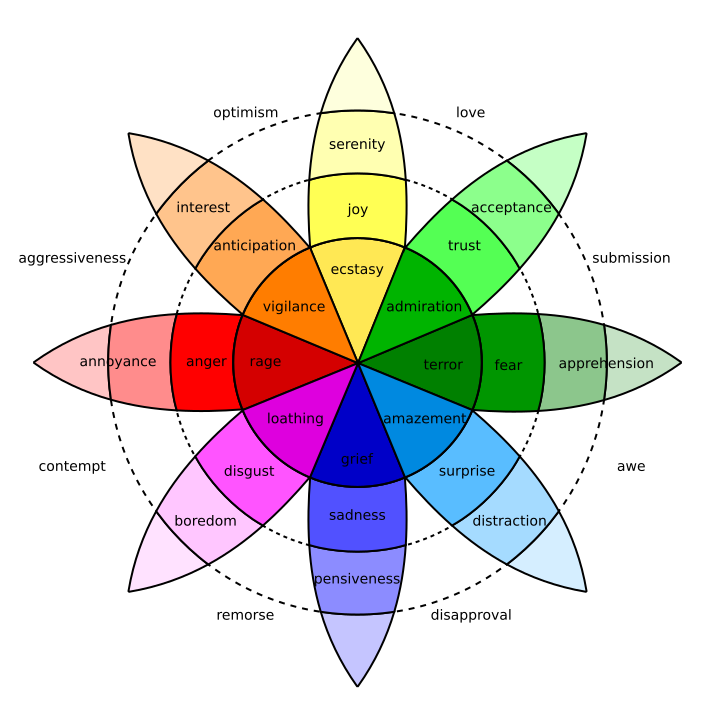
\includegraphics[width=10cm]{figures/plutchik-wheel.png}
\fcmfcaption{Koło emocji Plutchika \cite{plutchik1982psychoevolutionary}.}\label{rys:plutchik_wheel}
\end{figure}

Podsumowując wymienione modele emocji możemy wydzielić dwa główne typy: kategoryczne oraz wymiarowe. Modele wymiarowe mapują emocję w sposób ciągły na wektory. Modele kategoryczne klasyfikują emocję do konkretnej emocji dyskretnej, np. jednej z wybranego modelu emocji Ekmana lub Plutchika. Modele kategoryczne mają pewne wady. Jedną z nich jest brak możliwości opisania innych emocji oraz utrudnione opisywanie emocji złożonej z kilku różnych podtypów zdefiniowanych w dyskretnym modelu. Drugą wadą jest brak możliwości porównywania emocji, co umożliwiłby model wymiarowy, za pomocą porównywania dwóch wektorów. Wybór odpowiedniego modelu emocji nie jest łatwy, a jednocześnie jest bardzo ważnym elementem do późniejszej klasyfikacji emocji. Decydując się na kategoryczny typ emocji, z jednej strony mamy prosty model Ekmana który nie jest w stanie zamodelować złożonych emocji. Z drugiej strony w modelu Plutchika może być bardzo trudno rozróżnić drobnoziarniste emocje od siebie. Wybór ten należy zatem dokonać mając na uwadze wielkość oraz jakość zbioru danych.

\section{Głębokie uczenie}

W przetwarzaniu języka naturalnego z użyciem głębokich sieci neuronowych coraz częściej używane są techniki transferu wiedzy (ang. \textit{transfer learning}) oraz adaptacji domenowej. Model języka jest kluczowym elementem do zastosowania powyższych technik. Umożliwia on przewidzenie kontekstu w jakim dane słowo znajduje się w zdaniu i na tej podstawie umożliwia odkryć jego prawdziwy sens. Jest uważany za bardzo istotny element w dziedzinie \textit{NLP}, który stanowi podstawę do wszelkich zastosowań przetwarzania języka naturalnego. Najważniejsze jego cechy to zrozumienie długofalowych zależności i hierarchicznej struktury tekstu, a największe zalety to otwarte i wolne zasoby do jego stworzenia. Jest tworzony za pomocą nienadzorowanego procesu uczenia, który potrzebuje tylko korpusu nieoznakowanego tekstu.

Znakomitym przykładem użycia transferu wiedzy za pomocą wielokrotnego uczenia modelu języka jest metoda \textit{ULMFIT} \cite{howard2018universal} (ang. \textit{Universal Language Model Fine-tuning for Text Classification}, która może być zastosowana do każdego zadania w NLP. Zastosowane są w niej techniki, które są kluczowe dla dostrojenia modelu językowego. Używane są w niej 3 warstwy sieci neuronowej wykorzystującej komórki LSTM (ang. \textit{Long Short-Term Memory}), które w przeciwieństwie do standardowych komórek sieci neuronowych, posiadają połączenia zwrotne, umożliwiające zapamiętanie sąsiednich stanów w sieci. Dodatkowo zastosowana jest technika przerywania (ang. \textit{dropout}) niwelująca problem przeuczania. Cały etap nauki w metodzie \textit{ULMFIT} składa się z 3 etapów zaprezentowanych na rysunku \ref{rys:ulmfit}. Na początku następuje szkolenie wstępne modelu językowego na dowolnym korpusie, następnie dostrojenie modelu językowego na zadaniu docelowym i na końcu dostrojenie klasyfikatora na zadaniu docelowym. Dzięki zastosowaniu tych technik możliwe jest wyuczenie wstępne modelu języka na dowolnych danych, (np. korpus Wikipedii) a następnie wykorzystanie tego wstępnie wyuczonego modelu na zadaniu docelowym. Na podobnej zasadzie działają dzisiejsze najbardziej wyrafinowane architektury głębokich sieci neuronowych w zastosowaniu przetwarzania języka naturalnego nazywane aktualnym stanem techniki (ang. \textit{state of the art}).

\begin{figure}[t]
\centering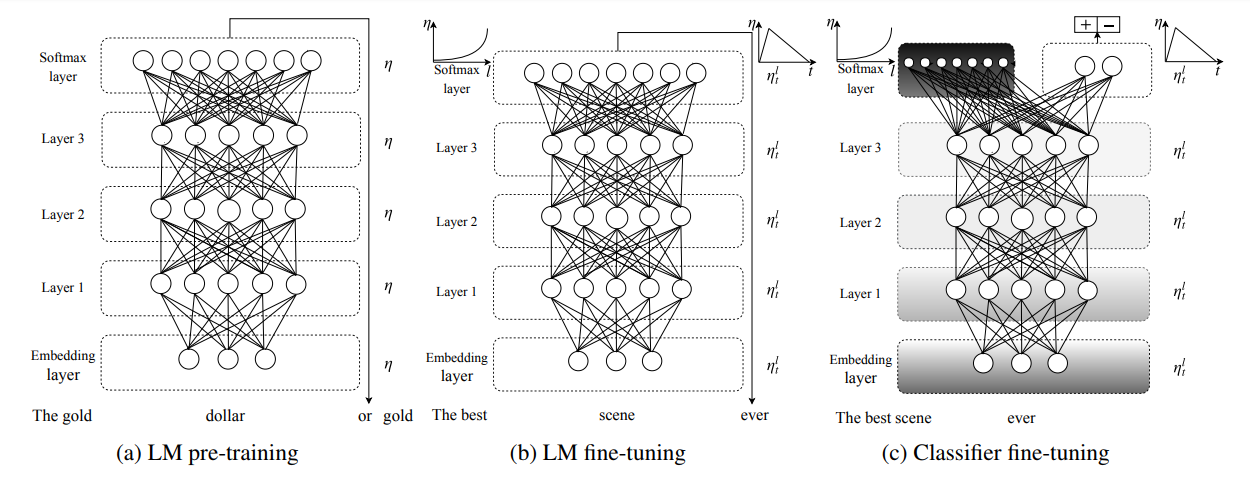
\includegraphics[width=\textwidth]{figures/ulmfit.png}
\fcmfcaption{3 etapy nauki modelu języka (ang. \textit{LM}) w metodzie ULMFIT \cite{howard2018universal}.}\label{rys:ulmfit}
\end{figure}
\chapter{Analiza eksploracyjna}

Rozdziały dokumentujące pracę własną studenta: opisujące ideę, sposób lub metodę 
rozwiązania postawionego problemu oraz rozdziały opisujące techniczną stronę rozwiązania 
--- dokumentacja techniczna, przeprowadzone testy, badania i uzyskane wyniki. 

Praca musi zawierać elementy pracy własnej autora adekwatne do jego wiedzy praktycznej uzyskanej w
okresie studiów. Za pracę własną autora można uznać np.: stworzenie aplikacji informatycznej lub jej
fragmentu, zaproponowanie algorytmu rozwiązania problemu szczegółowego, przedstawienie projektu 
np.~systemu informatycznego lub sieci komputerowej, analizę i ocenę nowych technologii lub rozwiązań
informatycznych wykorzystywanych w przedsiębiorstwach, itp. 

Autor powinien zadbać o właściwą dokumentację pracy własnej obejmującą specyfikację założeń i 
sposób realizacji poszczególnych zadań
wraz z ich oceną i opisem napotkanych problemów. W przypadku prac o charakterze 
projektowo-implementacyjnym, ta część pracy jest zastępowana dokumentacją techniczną i użytkową systemu. 

W pracy \textbf{nie należy zamieszczać całego kodu źródłowego} opracowanych programów. Kod źródłowy napisanych
programów, wszelkie oprogramowanie wytworzone i wykorzystane w pracy, wyniki przeprowadzonych
eksperymentów powinny być umieszczone np. na płycie CD, stanowiącej dodatek do pracy.

\section*{Styl tekstu}

Należy\footnote{Uwagi o stylu pochodzą częściowo ze stron prof. Macieja Drozdowskiego~\cite{zhong2019knowledgeenriched}.} 
stosować formę bezosobową, tj.~\emph{w pracy rozważono ......, 
w ramach pracy zaprojektowano ....}, a nie: \emph{w pracy rozważyłem, w ramach pracy zaprojektowałem}. 
Odwołania do wcześniejszych fragmentów tekstu powinny mieć następującą postać: ,,Jak wspomniano wcześniej, ....'', 
,,Jak wykazano powyżej ....''. Należy unikać długich zdań. 

Niedopuszczalne są zwroty używane w języku potocznym. W pracy należy używać terminologii informatycznej, która ma 
sprecyzowaną treść i znaczenie. 

Niedopuszczalne jest pisanie pracy metodą \emph{cut\&paste}, bo jest to plagiat i dowód intelektualnej indolencji autora.
Dane zagadnienie należy opisać własnymi słowami. Zawsze trzeba powołać się na zewnętrzne źródła. 

\chapter{Przetwarzanie danych}
\label{chapter:przetwarzanie_danych}

\section{Wczytanie i oczyszczenie danych}

Pierwszym etapem przygotowania danych do użycia w modelu jest ich wczytanie oraz przetworzenie. Zbiór danych z EmoContext zawiera pięć kolumn (rys. \ref{rys:examples_semeval}). W pierwszej kolumnie znajduje się identyfikator, w kolumnach od 2 do 4 zawarty jest docelowy tekst który będzie użyty jako wejście do modelu, a w ostatniej kolumnie znajduje się etykieta emocji. Po wczytaniu danych następuje połączenie trzech kolumn z tekstem w jeden ciąg znaków, oddzielone znakiem specjalnym \textit{EOS} (ang. \textit{end of sentence}). Jest to niezbędna operacja która umożliwi docelowemu modelowi oddzielić trzy wypowiedzi od siebie. Następnie na tak otrzymanym ciągu znaków wykonywane są operacje usuwania powtarzających się znaków interpunkcyjnych (np. \textit{"!!!!"} zostanie zamienione na pojedynczy znak \textit{"!"}). Na końcu wykonywane jest oddzielenie znaków interpunkcyjnych od wyrazów, usunięcie powtarzających się spacji oraz zamiana wszystkich dużych liter na małe.

Jest to wspólny proces dla wszystkich modeli, kolejne etapy zostały podzielone na te zastosowane do architektur korzystających z rekurencyjnych komórek LSTM oraz tych korzystających z architektury BERT. 

\section{Przetwarzanie dla architektur LSTM}

\subsection{Tokenizacja i wyrównanie}

Modele głębokie przetwarzania języka naturalnego nie operują na jawnym tekście w postaci ciągu znaków, tylko na reprezentacji w postaci liczbowej. Do reprezentacji wyrazów używane są słowniki które przechowują wszystkie znane słowa z korpusu uczącego. Do tej zamiany użyta została metoda \texttt{Tokenizer} z pakietu TensorFlow. Klasa ta pozwala na wektoryzację korpusu tekstu, poprzez przekształcenie każdego wyrazu w liczbę całkowitą. Każda z tych liczb odpowiada indeksowi tego słowa w słowniku.

Po przekształceniu każdego słowa w token następuje wyrównanie długości wszystkich przykładów w zbiorze. Przykładowa liczba użyta do wyrównania (ang. \textit{padding}) to 20. Wszystkie przykłady, które mają mniejszą liczbę tokenów, wypełniane są tokenem zerowym aż do osiągnięcia długości 20, a wszystkie przykłady które mają większą liczbę tokenów są skracane od końca. W ten sposób została utworzona macierz danych która może być wykorzystana do użycia w nauce i ewaluacji modeli.

\subsection{Zagłębienia słów}
\label{section:words_embeddings}

W przypadku głębokich sieci neuronowych z rekurencyjnymi komórkami LSTM wysoce efektywne jest użycie zagłębień słów (ang. \textit{words embeddings}) jako wejścia do pierwszej warstwy sieci neuronowej. Osadzanie słów jest przeprowadzone za pomocą mapowania tych słów na wektory liczb rzeczywistych. Reprezentacja słów jako wektory liczb jest rozszerzeniem reprezentacji \textit{jeden z N} (ang. \textit{one hot encodings}), która jest używana w celu zwiększenia wydajności modeli NLP. Jest to także możliwość użycia transferu wiedzy w postaci wstępnie wytrenowanych zagłębień słów jako reprezentacji danych wejściowych. Jednym z algorytmów, który umożliwia stworzenie takiej reprezentacji jest metoda GloVe  \cite{brochier2019global} (ang. \textit{Global Vectors for Word Representation}), stworzona przez zespół z Uniwersytetu Stanford. Udostępniona przez nich macierz umożliwia użycie tej reprezentacji, jako odwzorowanie słów na wektory liczb rzeczywistych. Słowa zmapowane w tej przestrzeni mają zachowane pewne właściwości, odległość między nimi jest powiązana z podobieństwem semantycznym. Na rysunku \ref{rys:visualize_glove} ukazane są przykładowe słowa i zachowane podobieństwo np. między słowami love i beautiful. Sposób uzyskania tej reprezentacji bazuje na współwystępowaniu danych słów w korpusie w otoczeniu które je definiuje. Główną intuicją tego modelu jest założenie, że proporcje prawdopodobieństwa współwystępowania słów mają potencjał do kodowania jakiejś formy znaczenia. Wynikiem tej metody są wektory słów które bardzo dobrze radzą sobie z zadaniami opartymi o podobieństwo, analogię, a także odkrywaniu semantyki emocjonalnej słów i wiele innych wymienionych w pakiecie \textit{word2vec} \cite{mikolov2013efficient}.

\begin{figure}[t]
\centering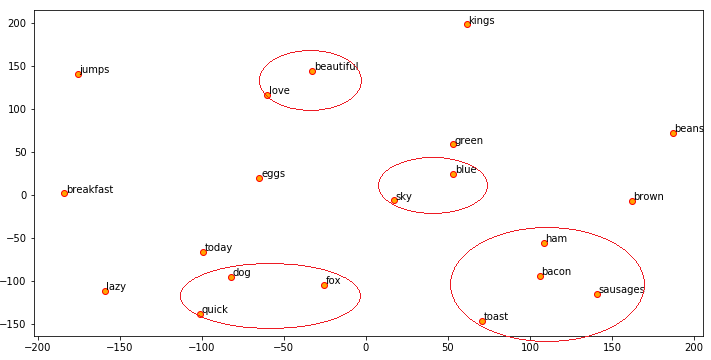
\includegraphics[width=\textwidth]{figures/visualize_glove.png}
\fcmfcaption{Przykładowe słowa w przestrzeni wektorowej GloVe  \cite{brochier2019global}.}\label{rys:visualize_glove}
\end{figure}

\section{Przetwarzanie dla architektur BERT}

\subsection{Tokenizacja, dodatkowe tokeny i wyrównanie}

Do utworzenia reprezentacji wejściowej dla architektury BERT niezbędne było dostosowanie się do wymagań dla tego modelu. Do przetworzenia tekstu na tokeny użyto klasę \texttt{BertTokenizer} z pakietu \texttt{transformers}. Umożliwia ona zamianę reprezentacji ciągu znaków na tokeny które są mapowane dzięki wbudowanemu słownikowi w architekturę BERT za pomocą algorytmu \textit{WordPiece} \cite{wu2016googles}.

Tokenizacja rozkłada się na kilka etapów, jednym z nich jest dodanie specjalnych tokenów oznaczających początek (\textit{[CLS]}) oraz separację (\textit{[SEP]}) kolejnych wypowiedzi, widocznych jako Input na rysunku \ref{rys:bert_token}. Następnie wydzielone tokeny mapowane są na identyfikatory za pomocą wbudowanego słownika. W ten sposób otrzymane reprezentacje zdań zostają wyrównane do danej szerokości i przekazane do wygenerowania maski uwagi o tej samej szerokości co wyrównane zdanie. Ma to na celu wskazanie na których miejscach w zdaniu występują tokeny należące do zdania za pomocą liczby 1. Te tokeny w zdaniu które były sztucznie dodane dla celów wyrównania otrzymują liczbę 0. Tak otrzymana reprezentacja zostanie przekazana na wejście modelu korzystającego z architektury BERT.

\begin{figure}[t]
\centering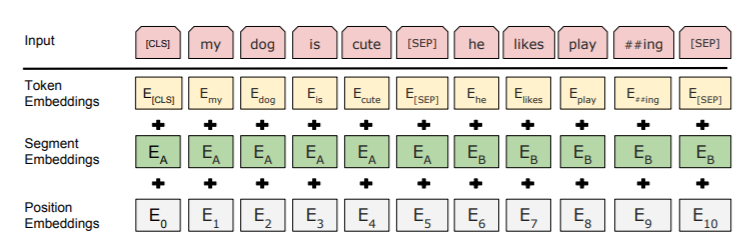
\includegraphics[width=\textwidth]{figures/bert_token.png}
\fcmfcaption{Przykładowe zdanie zamienione na reprezentację BERT \cite{devlin2018bert}.}\label{rys:bert_token}
\end{figure}
\chapter{Budowa modeli}

\section{Jednowarstwowa architektura LSTM}
\label{section:one_lstm}

Pierwszy model bazuje na zaproponowanej przez organizatorów konkursu jednowarstwowej architekturze sieci rekurencyjnej z komórkami LSTM. Zastosowanie tej budowy modelu zapewnia zdolność do uczenia się długoterminowych zależności przy jednoczesnym unikaniu długotrwałego problemu uzależnienia. 

Przygotowawczym etapem modelu jest przedstawienie wymagań dla danych, które mogą być przetwarzane w warstwie wejściowej (ang. \textit{Input Layer}). Każdy przykład jest przetworzony zgodnie z opisem w rozdziale \ref{chapter:przetwarzanie_danych}. Jednym z ostatnich etapów przetwarzania jest wyrównanie wszystkich przykładów do równej długości w tym przypadku 200, zgodnie z rysunkiem \ref{rys:lstm_one_graph} przedstawiającym budowę jednowarstwowej architektury LSTM.

\begin{figure}[t]
\centering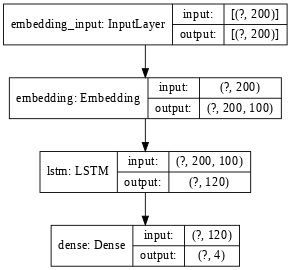
\includegraphics[width=6cm]{figures/reports/lstm_one_graph.png}
\fcmfcaption{Graf przedstawiający budowę jednowarstwowej architektury LSTM.}\label{rys:lstm_one_graph}
\end{figure}

Kolejną warstwą jest zamiana reprezentacji słowa na gęstą reprezentację wektorową opisaną w sekcji \ref{section:words_embeddings}. Do uzyskania tej reprezentacji użyto gotowe macierze udostępnione przez autorów metody na stronie internetowej\footnote{\url{https://nlp.stanford.edu/projects/glove/}}. Do wyboru były macierze przygotowane na różnych zbiorach danych oraz o różnych szerokościach wektorów. Testy przeprowadzono z użyciem zagłębień słów wytrenowanych na zbiorze danych pochodzących z Wikipedii oraz z archiwum danych tekstowych Gigaword 5 (ang. \textit{English Gigaword Fifth Edition}). Wybór szerokości wektorów podyktowany był złożonością modelu i czasem nauki, z pośród zbioru 50, 100, 200, 300 zdecydowano się na szerokość 100. Podsumowując złożoność tego etapu zawiera on prawie 2 miliony wewnętrznych parametrów, które są zamrożone na czas uczenia. Rysunek \ref{rys:lstm_one_table} przedstawia szczegóły budowy jednowarstwowej architektury LSTM, wraz z tą warstwą o nazwie \textit{Embedding}.

\begin{figure}[t]
\centering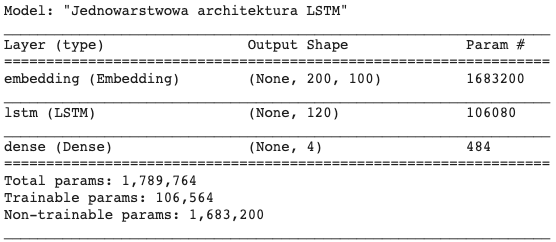
\includegraphics[width=10cm]{figures/reports/lstm_one_table.png}
\fcmfcaption{Tabela przedstawiająca szczegóły budowy jednowarstwowej architektury LSTM.}\label{rys:lstm_one_table}
\end{figure}

Do stworzenia kolejnej warstwy użyto gotową reprezentację LSTM z pakietu tensorflow o nazwie \textit{keras.layers.LSTM}, która udostępnia możliwość definiowania konkretnych szczegółów implementacyjnych. W warstwie tej użyto domyślną funkcję aktywacji tangens hiperboliczny. Po obserwacji krzywej uczenia reprezentującej dokładność oraz wartość funkcji straty zauważono zjawisko przeuczenia. Dokładność dla zbioru uczącego rosła wraz z malejącą dokładnością dla zbioru walidacyjnego. Z tego powodu zdecydowano się na użycie metody przerywania (ang. \textit{dropout}), zdefiniowanej w tej warstwie. Pomogło to zmniejszyć wpływ zjawiska przeuczania się modelu.

Ostatnim etapem jest wybór odpowiedniej klasy za pomocą warstwy jednokierunkowej. Wyjście z poprzedniej warstwy nazywane stanem ukrytym (ang. \textit{hidden state}) o szerokości 120 jest gęsto połączone z 4 neuronami decydującymi odpowiednio o każdej z kolejnych etykiet emocji. Jako funkcję aktywacji tej warstwy, zgodnie z sugestią organizatorów konkursu użyto funkcję sigmoidalną. Zauważona jednak została niekompatybilność tej funkcji z konkretnym zastosowaniem dla klasyfikacji wieloklasowej co zostało poprawione w kolejno zaprezentowanych modelach.  

Ostatnim elementem budowy tego modelu jest wybór algorytmu optymalizacyjnego. Wybrano algorytm RMSprop \cite{ruder2016overview} (ang. \textit{Root Mean Square Propagation}), który dobrze radzi sobie z wygasającymi wskaźnikami uczenia oraz przeciwdziała obliczeniowym problemom numerycznym. Jako funkcję straty użyto \textit{Categorical Cross-Entropy loss}, która bardzo dobrze radzi sobie w problemach klasyfikacji wielu klas.

\section{Głęboka architektura LSTM}

Głęboka architektura LSTM jest rozszerzeniem architektury jednowarstwowej opisanej w punkcie \ref{section:one_lstm}. Głównym celem było porównanie złożoności architektury płytkiej i głębokiej oraz wpływ rozszerzenia modelu o kolejne warstwy na wynik. Modyfikacje polegały przede wszystkim na dodaniu kolejnych warstw oraz lekkie modyfikacje parametrów oraz funkcji wewnątrz modelu. Pierwsze dwie warstwy, wejściowa (\textit{Input Layer}) oraz mapująca słowa na gęstą reprezentację wektorową (\textit{Embedding}) zostały bez zmian.

Do rozszerzenia jednowarstwowej części sieci rekurencyjnej zamiast zwykłych komórek LSTM użyto dwukierunkowych komórek LSTM. Z założenia rozszerzenie to powinno poprawić wydajność modelu przy problemach z klasyfikacją sekwencji \cite{ding2018densely}. W tym przypadku można było użyć tego rozszerzenia ponieważ od razu są dostępne wszystkie sekwencje czasowe sekwencji wejściowej. W tym momencie dwukierunkowe komórki LSTM łączą dwie ukryte warstwy o przeciwnych kierunkach. Dzięki tej formie uczenia warstwa wyjściowa może jednocześnie uzyskiwać informacje z przeszłych jak i przyszłych stanów, co nie było możliwe przy użyciu podstawowych komórek LSTM. Zabieg ten pomaga lepiej zrozumieć kontekst gdyż znaczenie danego słowa może zależeć także od słów, które są przed danym słowem. Dodatkowo zamiast jednej warstwy sieci rekurencyjnej użyto łącznie trzy warstwy używające dwukierunkowego LSTM. Pierwsze dwie warstwy na wyjściu oprócz ukrytego stanu zwracają także sekwencję o długości 200, którą przekazują na wejście kolejnej warstwy sieci LSTM. Widać to na rysunku \ref{rys:lstm_deep_graph}, który przedstawia graf głębokiej architektury LSTM.

\begin{figure}[t]
\centering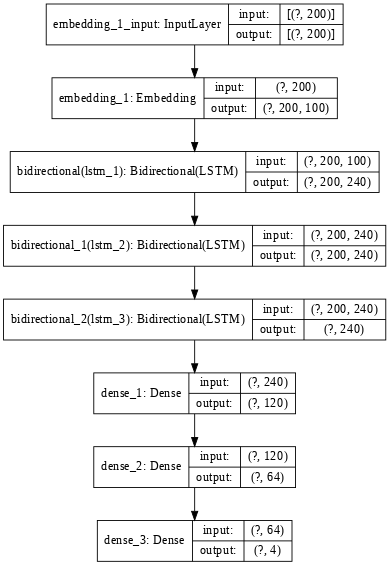
\includegraphics[width=8cm]{figures/reports/lstm_deep_graph.png}
\fcmfcaption{Graf przedstawiający budowę głębokiej architektury LSTM.}\label{rys:lstm_deep_graph}
\end{figure}

Kolejną modyfikacją było dodanie kolejnych warstw sieci gęstej. Wcześniej użytą jedną warstwę zawierającą 4 neurony wyjściowe rozszerzono o kolejne dwie warstwy gęste. Pierwsza z nich zawiera 120 neuronów a druga zawiera 64 neurony. Szczegóły tej budowy przedstawiono na rysunku \ref{rys:lstm_deep_table}, który przestawia tabelę prezentującą szczegóły budowy głębokiej architektury LSTM. Do dodanych warstw użyto innej funkcji aktywacji jaką jest jednostronnie obcięta funkcja liniowa (ang. \textit{ReLU}), która stała się standardem do użycia w wewnętrznych warstwach gęstej sieci neuronowej \cite{xu2015empirical}. W ostatniej warstwie także zamieniono funkcję aktywacji na funkcję \textit{softmax}, która lepiej nadaje się do klasyfikacji wieloklasowej.

\begin{figure}[t]
\centering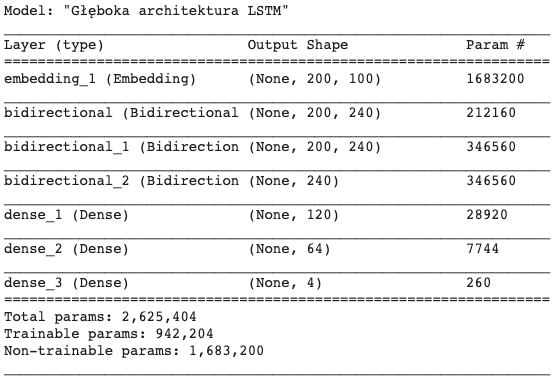
\includegraphics[width=10cm]{figures/reports/lstm_deep_table.png}
\fcmfcaption{Tabela przedstawiająca szczegóły budowy głębokiej architektury LSTM.}\label{rys:lstm_deep_table}
\end{figure}

Porównując dokonane rozszerzenia modelu z jedną warstwą LSTM, oraz wykonując opisane modyfikacje warstw zwiększyła się złożoność modelu. Prostym sposobem na porównanie modeli jest sprawdzenie liczby parametrów, które definiują zachowanie sztucznych neuronów, inaczej nazywane wagami neuronu. W tabeli \ref{tab:tabela_modele} przedstawione są liczby parametrów podzielonych na dwie grupy. Parametry trenowalne modelu to są wagi, które ulegają modyfikacji, liczba tych parametrów zwiększyła się około dziewięciokrotnie co ilustruję skalę zmian. Parametry stałe to są wagi użyte do generacji gęstych reprezentacji wektorowych, które były zamrożone na czas nauki modeli.  

\begin{table}[t]
\fcmtcaption{Tabela porównująca szczegóły budowy poszczególnych model.}\label{tab:tabela_modele}
\centering\footnotesize%
\begin{tabular}{c c c c}
\toprule
model & parametry trenowalne & parametry stałe & SUMA \\
\midrule
Jednowarstwowy LSTM   & 106,564 & 1,683,200 & 1,789,764 \\
Głęboki LSTM   & 942,204 & 1,683,200 & 2,625,404 \\
BERT todo   & xx & xx & xxx \\
\bottomrule
\end{tabular}
\end{table}

% \section{Głęboka architektura BERT}

% TODO \cite{devlin2018bert} BERT
\chapter{Ewaluacja modeli}

\section{Dobór parametrów}

Proces nauki poszczególnych modeli rozpoczęto od zdefiniowania \textit{hiper-parametrów} \cite{probst2018tunability}. Są to parametry, których wartości są ustawione przed rozpoczęciem procesu uczenia się i definiują one zachowanie poszczególnych warstw modelu. Początkowe wartości tych parametrów zdefiniowano zgodnie z powszechnymi wartościami używanymi w podobnych architekturach oraz na podstawie załączonej literatury. Dalsze kroki polegały na dostosowaniu tych parametrów do osiągnięcia najlepszego wyniku. Dobrym sposobem na znalezienie optymalnego doboru parametrów są metody typu wyszukiwanie w siatce (ang. \textit{grid search}) oraz wyszukiwanie losowe (ang. \textit{random search}) \cite{liashchynskyi2019grid}. Polegają one na porównywaniu działania modelu z przyjętymi parametrami wybranymi z przestrzeni parametrów. Podjęto próby użycia tych metod, jednak ze względu na ograniczone zasoby obliczeniowe oraz długi czas przetwarzania ograniczono przestrzeń parametrów do minimum. Pozwoliło to na przeszukanie bardzo małego zbioru wartości co i tak dało satysfakcjonujące wyniki.

\subsection{Parametry modeli LSTM}

Dobrane wartości dla modeli jednowarstwowego LSTM \ref{section:one_lstm} oraz głębokiego LSTM \ref{section:deep_lstm} przedstawiono w tabeli \ref{tab:parametry_lstm}. Założenie użycia tych samych hiper-parametrów dla obu modeli było sprawdzenie wpływu głębokości (liczby warstw) modelu na wynik. Rozmiar LSTM dotyczy liczby komórek LSTM w jednej warstwie, dobór wartości 120 zależał od wielkości zbioru danych oraz od ograniczeń zasobowych. Parametr przerywania (ang. \textit{dropout}) użyty do przeciwdziałania przeuczania się modelu został wybrany z pośród dwóch wartości 0.2 oraz 0.5, okazało się że 0.2 ma lepszy wpływ na wynik. Rozmiar wektora słów dotyczy szerokości gęstej reprezentacji wektorowej każdego słowa, czym większa wartość tym więcej informacji przenoszonej przez te wektory, jednak ograniczenia zasobów pozwoliły na szerokość 100, gdzie maksymalna dostępna szerokość to 300. Pozostałe parametry dotyczą sposobu nauki modeli oraz szybkości i długości tego procesu, wartości te pozostały domyślne.

\begin{table}[t]
\fcmtcaption{Tabela prezentująca wybrane \textit{hiper-parametry} modeli korzystających z LSTM.}\label{tab:parametry_lstm}
\centering\footnotesize%
\begin{tabular}{l c}
\toprule
\textit{hiper-parametr} & wartość \\
\midrule
rozmiar LSTM   & 120 \\
wskaźnik uczenia się   & 0.003 \\
przerywanie (ang. \textit{dropout})   & 0.2 \\
liczba epok   & 100 \\
rozmiar wektora słów   & 100 \\
wielkość grupy (ang. \textit{batch}) & 200 \\
\bottomrule
\end{tabular}
\end{table}

\subsection{Parametry modeli BERT}

TODO

TODO

TODO

\section{Przebieg nauki}

Do procesu nauki użyto platformę \textit{Colab}\footnote{\url{https://colab.research.google.com/}}, która umożliwia korzystanie z zasobów karty graficznej (GPU) umożliwiającej dużo wydajniejszy proces nauki modeli. Dla jednowarstwowego LSTM czas przetwarzania jednej epoki to około 9 sekund, a dla modelu głębokiego LSTM to 64 sekundy. Przy użyciu laptopa czasy te były prawie dziesięciokrotnie większe co uniemożliwiło by tak sprawne projektowanie i dostrajanie modeli.

\subsection{Nauka modeli LSTM}

Proces nauki rozpoczęto od podstawowego modelu jednowarstwowego LSTM. Po doborze hiper-parametrów związanych z architekturą modelu dobrane były odpowiednie wartości dla liczby epok oraz wskaźnika uczenia się. Zauważono że po dwudziestej epoce dokładność przekroczyła 90\%, a po setnej epoce poprawa wyników była na tyle niewielka że przerwano proces nauki. Ostateczne wyniki są przedstawione na wykresach \ref{rys:lstm_one_deep_comparison} przedstawiających przebieg nauki dla modeli jednowarstwowego LSTM oraz głębokiego LSTM. W początkowych etapach nauki wartości funkcji straty (ang. \textit{loss}) oraz dokładności (ang. \textit{accuracy}) były bardzo podobne, jednak po dziesiątej epoce widać przewagę modelu głębokiego LSTM oznaczonego kolorem pomarańczowym. Wynikać to może z dużo większej złożoności tego modelu oraz możliwości zapamiętania przez ten model większej liczby cech przechowywanych w tekście.

\begin{figure}[t]
\centering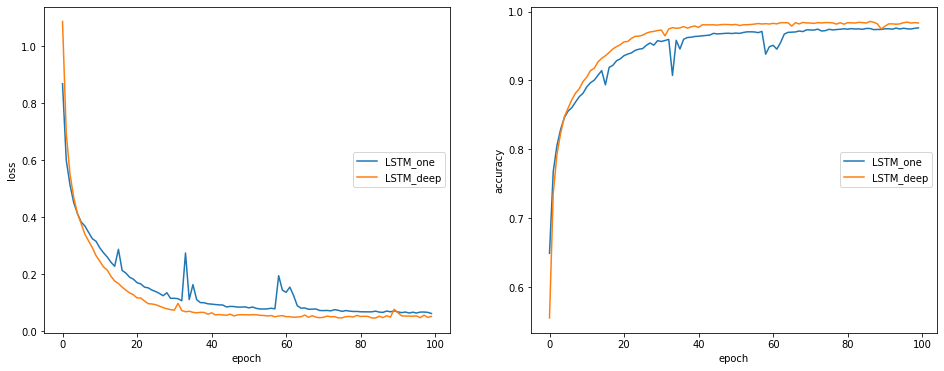
\includegraphics[width=\textwidth]{figures/reports/lstm_one_deep_comparison.png}
\fcmfcaption{Wykresy przedstawiające przebieg nauki dla modeli jednowarstwowego LSTM oraz głębokiego LSTM}\label{rys:lstm_one_deep_comparison}
\end{figure}

\subsection{Nauka modeli BERT}

TODO

TODO

TODO

\section{Metryki}

\subsection{Macierz pomyłek}

W dziedzinie sieci neuronowych oraz oceny jakości modeli uczenia maszynowego, a w szczególności w problemach klasyfikacji często pomocna jest macierz pomyłek, inaczej nazywana macierzą błędów. Jest to specyficzny układ tabel, który pozwala na wizualizację wydajności algorytmu. Składa się on z dwóch wymiarów: rzeczywistym i przewidywanym. Podaje on liczbę wyników prawdziwie dodatnich (\textit{TP}), prawdziwie ujemnych (\textit{TN}), fałszywie dodatnich (\textit{FP}) oraz fałszywie ujemnych(\textit{FN}).

\begin{table}[ht]
\fcmtcaption{Tabela ukazująca macierz pomyłek.}\label{tab:tabela_matrix}
\centering\footnotesize%
\begin{tabular}{l|l|c|c|}
\multicolumn{2}{c}{}&\multicolumn{2}{c}{Prawdziwa etykieta}\\
\cline{3-4}
\multicolumn{2}{c|}{}&Positive&Negative\\
\cline{2-4}
\multirow{2}{*}{Przewidziana etykieta} & Positive & $TP$ & $FP$\\
\cline{2-4}
& Negative & $TN$ & $FN$\\
\cline{2-4}
\multicolumn{1}{c}{} & \multicolumn{1}{c}{Łącznie} & \multicolumn{1}{c}{$P$} & \multicolumn{1}{c}{$N$}\\
\end{tabular}
\end{table}

Pozwala to na bardziej szczegółową analizę oraz formułowanie wielu metryk na podstawie wartości z tej macierzy. Niektóre z tych miar zastosowano do ewaluacji modeli i zaprezentowano w kolejnych podsekcjach.

\subsection{Miara jakości nauki}

Główną metryką analizowaną w trakcie nauki modelu była dokładność (ang. \textit{accuracy}), zdefiniowana w poniższym równaniu \ref{eqn:accuracy}.

\begin{equation}
\label{eqn:accuracy}
dokladnosc=\frac{TP + TN}{P + N}
\end{equation}

Miara ta odwzorowuje efektywność nauki. Podczas jej obserwacji można stwierdzić czy każda kolejna epoka nauki poprawia wynik, czy też go pogarsza. Zbiór danych treningowy miał zrównoważony rozkład klas na tyle, że zastosowanie tej metryki miało sens. Niestety jeśli zestaw danych mocno niezbalansowany, tak jak w przypadku zbioru testowego miara ta może wprowadzić w błąd. Z tego powodu zastosowanie tej metryki ograniczono tylko do obserwacji procesu nauki, a ostateczną ocenę modelu wykonano na podstawie innych miar.

\subsection{Ostateczna ocena modelu}

Ostateczną ocenę modelu dokonano za pomocą obliczenia mikro średniego wyniku F1 dla trzech klas emocji \textit{Happy}, \textit{Sad}, \textit{Angry}. Wybór ten wynika z niezbalansowania klas w zbiorze testowym oraz dominacją występowania etykiety \textit{Others}, którą pominięto w ostatecznej ocenie. Wynik F1 jest średnią harmoniczną precyzji i czułości, zdefiniowanych w poniższych wzorach. Końcowy wynik uzyskany jest poprzez uśrednianie w skali mikro, na podstawie częstotliwości klas występujących w zbiorze treningowym. Poniższe wzory przedstawiają poszczególne składniki oraz samą funkcję F1.

\begin{equation}
\label{eqn:precyzja}
precyzja = \frac{TP}{FP+TP}
\end{equation}

\begin{equation}
\label{eqn:czułość}
czulosc = \frac{TP}{FP+TP}
\end{equation}

\begin{equation}
\label{eqn:f1}
F1 = \frac{2 \cdot precyzja\cdot czulosc}{precyzja + czulosc}
\end{equation}

\section{Wyniki}

Jakość wyuczonych modeli na zbiorze treningowym porównano poprzez ewaluację predykcji tych modeli na zbiorze testowym. Głównymi założeniami porównań było sprawdzenie wpływu liczby warstw sieci neuronowej na wynik oraz porównanie tradycyjnych rekurencyjnych warstw do bardziej złożonych architektur jakim jest BERT. 

Porównanie jednowarstwowej architektury LSTM  z głęboką architekturą LSTM pokazuje przewagę dla modelu głębokiego. Większa liczba warstw pomogła osiągnąć lepszy wynik miary mikro F1, jednak jest to niewielka poprawa. Można spekulować że jednowarstwowa sieć LSTM dla tego zbioru danych była wystarczająca aby osiągnąć maksimum możliwości tej architektury. Z drugiej strony użycie gęstej reprezentacji wektorowej każdego słowa mogło ograniczyć możliwości warstw LSTM i spowodować że użycie kolejnych warstw sieci pomogło na zniwelowanie tylko małych błędów. Niestety analiza wpływu na wynik poszczególnych elementów sieci neuronowej jest utrudniona co uniemożliwia wyciągnięcie jasnych i sprawdzonych wniosków.

TODO BERT

TODO

TODO

TODO

\begin{table}[ht]
\fcmtcaption{Tabela pokazująca wyniki poszczególnych modeli.}\label{tab:tabela_results}
\centering\footnotesize%
\begin{tabular}{c c c c c}
\toprule
model & dokładność & mikro precyzja & micro czułość & \textbf{mikro F1} \\
\midrule
Jednowarstwowy LSTM & 0.85 & 0.49 & 0.70 & 0.58 \\
Głęboki LSTM & 0.87 & 0.51 & 0.71 & 0.60 \\
BERT & \textbf{0.90} & \textbf{0.57} & \textbf{0.81} & \textbf{0.67} \\
\bottomrule
\end{tabular}
\end{table}
\chapter{Podsumowanie}

Celem pracy było opracowanie modelu uczenia maszynowego opartego na głębokich sieciach neuronowych w celu detekcji emocji w dialogach. W jego ramach zostały zaprojektowane oraz przetestowane trzy różne architektury sieci neuronowych oraz została przeprowadzona analiza porównawcza tych modeli. Ponad to wszystkie zadania, które były niezbędne do zrealizowania tego celu także zostały wykonane. Są to między innymi zadania zapoznania się z literaturą dotyczącą głębokich sieci neuronowych i modeli emocji, przegląd oraz zapoznanie się z dostępnymi frameworkami do uczenia głębokiego, wstępna analiza wybranego zbioru danych oraz ewaluacja stworzonych modeli.

Rozpoznawanie emocji z tekstu jest zadaniem, które wymaga wielu czynników do poprawnego zrozumienia danego przekazu. Aby móc odkryć właściwą etykietę emocji należy spojrzeć na przekaz jako na całość, a nie na pojedyncze wyrazy, które mogą nieść inne znaczenie w różnych kontekstach. W podobny sposób objawia się działanie przedstawionych architektur do zrozumienia języka pisanego. Tradycyjne sieci neuronowe, proste metody uczenia maszynowego lub metody zliczające nie są w stanie odkryć znaczenia wypowiedzi jako całości. Bardzo ważnym elementem jest zrozumienie kontekstu oraz poradzenie sobie z problemami takimi jak występowanie sarkazmu lub ukrytego znaczenia.

Architektury korzystające z rekurencyjnych komórek LSTM są skonstruowane do rozumienia długotrwałych zależności i połączeń między wyrazami występującymi w zdaniu. Dzięki nim można było odkryć znaczenie przekazu, które zależało od kilku poprzednich wypowiedzi. Jeszcze lepsza okazała się architektura korzystająca z modelu BERT. Zastosowane w niej mechanizmy samoobserwacji oraz złożona budowa pozwoliła na jeszcze dokładniejsze zrozumienie tekstu.

Największym problemem w trakcie realizacji projektu okazały się ograniczenia zasobowe oraz długi czas przetwarzania modeli. Korzystanie z lokalnego laptopa do przeprowadzenia obliczeń oraz nauki modeli okazał się procesem zbyt długotrwałym oraz powodującym dużą zajętość zasobów takich jak pamięć oraz procesor. Pomocne okazały się serwisy udostępniające moce obliczeniowe w chmurze. Platforma Colab, użyta do trenowania modeli udostępniała dodatkowo dostęp do kart graficznych umożliwiających jeszcze efektywniejsze trenowanie modeli.

Do realizacji pracy użyto tylko niektórych z najbardziej popularnych metod głębokiego uczenia. W trakcie realizacji pracy wydano najnowszą architekturę określaną jako nowy stan techniki w przetwarzaniu języka naturalnego \textit{GPT-3} \cite{brown2020language}. Do uzyskania jeszcze lepszych wyników warto by przetestować działanie podobnych architektur oraz poświęcić więcej czasu na lepszym doborze parametrów. Istnieje także możliwość rozwijania obecnych architektur o inne zbiory danych oraz dostosowanie ich do użycia w praktyce w prawdziwych systemach informatycznych.

%--------------------------------------
% Literatura
%--------------------------------------

\bibliographystyle{plain}{\raggedright\sloppy\small\bibliography{bibliografia}}

%--------------------------------------
% Dodatki
%--------------------------------------

% EDIT: Te 3 linijki nie były zakomentowane, te nowe page może trzeba bedzie odkomentować
% \cleardoublepage\appendix%
% \newpage
% \chapter{Płyta CD}

Płyta CD z elektroniczną wersją pracy, stworzonym projektem oraz danymi wejściowymi.

%--------------------------------------
% Informacja o prawach autorskich
%--------------------------------------

\ppcolophon

\end{document}
